
%% bare_conf.tex
%% V1.3
%% 2007/01/11
%% by Michael Shell
%% See:
%% http://www.michaelshell.org/
%% for current contact information.
%%
%% This is a skeleton file demonstrating the use of IEEEtran.cls
%% (requires IEEEtran.cls version 1.7 or later) with an IEEE conference paper.
%%
%% Support sites:
%% http://www.michaelshell.org/tex/ieeetran/
%% http://www.ctan.org/tex-archive/macros/latex/contrib/IEEEtran/
%% and
%% http://www.ieee.org/

%%*************************************************************************
%% Legal Notice:
%% This code is offered as-is without any warranty either expressed or
%% implied; without even the implied warranty of MERCHANTABILITY or
%% FITNESS FOR A PARTICULAR PURPOSE!
%% User assumes all risk.
%% In no event shall IEEE or any contributor to this code be liable for
%% any damages or losses, including, but not limited to, incidental,
%% consequential, or any other damages, resulting from the use or misuse
%% of any information contained here.
%%
%% All comments are the opinions of their respective authors and are not
%% necessarily endorsed by the IEEE.
%%
%% This work is distributed under the LaTeX Project Public License (LPPL)
%% ( http://www.latex-project.org/ ) version 1.3, and may be freely used,
%% distributed and modified. A copy of the LPPL, version 1.3, is included
%% in the base LaTeX documentation of all distributions of LaTeX released
%% 2003/12/01 or later.
%% Retain all contribution notices and credits.
%% ** Modified files should be clearly indicated as such, including  **
%% ** renaming them and changing author support contact information. **
%%
%% File list of work: IEEEtran.cls, IEEEtran_HOWTO.pdf, bare_adv.tex,
%%                    bare_conf.tex, bare_jrnl.tex, bare_jrnl_compsoc.tex
%%*************************************************************************

% *** Authors should verify (and, if needed, correct) their LaTeX system  ***
% *** with the testflow diagnostic prior to trusting their LaTeX platform ***
% *** with production work. IEEE's font choices can trigger bugs that do  ***
% *** not appear when using other class files.                            ***
% The testflow support page is at:
% http://www.michaelshell.org/tex/testflow/



% Note that the a4paper option is mainly intended so that authors in
% countries using A4 can easily print to A4 and see how their papers will
% look in print - the typesetting of the document will not typically be
% affected with changes in paper size (but the bottom and side margins will).
% Use the testflow package mentioned above to verify correct handling of
% both paper sizes by the user's LaTeX system.
%
% Also note that the "draftcls" or "draftclsnofoot", not "draft", option
% should be used if it is desired that the figures are to be displayed in
% draft mode.
%
\documentclass[conference]{IEEEtran}
% Add the compsoc option for Computer Society conferences.
%
% If IEEEtran.cls has not been installed into the LaTeX system files,
% manually specify the path to it like:
% \documentclass[conference]{../sty/IEEEtran}





% Some very useful LaTeX packages include:
% (uncomment the ones you want to load)


% *** MISC UTILITY PACKAGES ***
%
%\usepackage{ifpdf}
% Heiko Oberdiek's ifpdf.sty is very useful if you need conditional
% compilation based on whether the output is pdf or dvi.
% usage:
% \ifpdf
%   % pdf code
% \else
%   % dvi code
% \fi
% The latest version of ifpdf.sty can be obtained from:
% http://www.ctan.org/tex-archive/macros/latex/contrib/oberdiek/
% Also, note that IEEEtran.cls V1.7 and later provides a builtin
% \ifCLASSINFOpdf conditional that works the same way.
% When switching from latex to pdflatex and vice-versa, the compiler may
% have to be run twice to clear warning/error messages.






% *** CITATION PACKAGES ***
%
%\usepackage{cite}
% cite.sty was written by Donald Arseneau
% V1.6 and later of IEEEtran pre-defines the format of the cite.sty package
% \cite{} output to follow that of IEEE. Loading the cite package will
% result in citation numbers being automatically sorted and properly
% "compressed/ranged". e.g., [1], [9], [2], [7], [5], [6] without using
% cite.sty will become [1], [2], [5]--[7], [9] using cite.sty. cite.sty's
% \cite will automatically add leading space, if needed. Use cite.sty's
% noadjust option (cite.sty V3.8 and later) if you want to turn this off.
% cite.sty is already installed on most LaTeX systems. Be sure and use
% version 4.0 (2003-05-27) and later if using hyperref.sty. cite.sty does
% not currently provide for hyperlinked citations.
% The latest version can be obtained at:
% http://www.ctan.org/tex-archive/macros/latex/contrib/cite/
% The documentation is contained in the cite.sty file itself.






% *** GRAPHICS RELATED PACKAGES ***
%
\ifCLASSINFOpdf
  % \usepackage[pdftex]{graphicx}
  % declare the path(s) where your graphic files are
  % \graphicspath{{../pdf/}{../jpeg/}}
  % and their extensions so you won't have to specify these with
  % every instance of \includegraphics
  % \DeclareGraphicsExtensions{.pdf,.jpeg,.png}
\else
  % or other class option (dvipsone, dvipdf, if not using dvips). graphicx
  % will default to the driver specified in the system graphics.cfg if no
  % driver is specified.
  % \usepackage[dvips]{graphicx}
  % declare the path(s) where your graphic files are
  % \graphicspath{{../eps/}}
  % and their extensions so you won't have to specify these with
  % every instance of \includegraphics
  % \DeclareGraphicsExtensions{.eps}
\fi
% graphicx was written by David Carlisle and Sebastian Rahtz. It is
% required if you want graphics, photos, etc. graphicx.sty is already
% installed on most LaTeX systems. The latest version and documentation can
% be obtained at:
% http://www.ctan.org/tex-archive/macros/latex/required/graphics/
% Another good source of documentation is "Using Imported Graphics in
% LaTeX2e" by Keith Reckdahl which can be found as epslatex.ps or
% epslatex.pdf at: http://www.ctan.org/tex-archive/info/
%
% latex, and pdflatex in dvi mode, support graphics in encapsulated
% postscript (.eps) format. pdflatex in pdf mode supports graphics
% in .pdf, .jpeg, .png and .mps (metapost) formats. Users should ensure
% that all non-photo figures use a vector format (.eps, .pdf, .mps) and
% not a bitmapped formats (.jpeg, .png). IEEE frowns on bitmapped formats
% which can result in "jaggedy"/blurry rendering of lines and letters as
% well as large increases in file sizes.
%
% You can find documentation about the pdfTeX application at:
% http://www.tug.org/applications/pdftex





% *** MATH PACKAGES ***
%
%\usepackage[cmex10]{amsmath}
% A popular package from the American Mathematical Society that provides
% many useful and powerful commands for dealing with mathematics. If using
% it, be sure to load this package with the cmex10 option to ensure that
% only type 1 fonts will utilized at all point sizes. Without this option,
% it is possible that some math symbols, particularly those within
% footnotes, will be rendered in bitmap form which will result in a
% document that can not be IEEE Xplore compliant!
%
% Also, note that the amsmath package sets \interdisplaylinepenalty to 10000
% thus preventing page breaks from occurring within multiline equations. Use:
%\interdisplaylinepenalty=2500
% after loading amsmath to restore such page breaks as IEEEtran.cls normally
% does. amsmath.sty is already installed on most LaTeX systems. The latest
% version and documentation can be obtained at:
% http://www.ctan.org/tex-archive/macros/latex/required/amslatex/math/





% *** SPECIALIZED LIST PACKAGES ***
%
%\usepackage{algorithmic}
% algorithmic.sty was written by Peter Williams and Rogerio Brito.
% This package provides an algorithmic environment fo describing algorithms.
% You can use the algorithmic environment in-text or within a figure
% environment to provide for a floating algorithm. Do NOT use the algorithm
% floating environment provided by algorithm.sty (by the same authors) or
% algorithm2e.sty (by Christophe Fiorio) as IEEE does not use dedicated
% algorithm float types and packages that provide these will not provide
% correct IEEE style captions. The latest version and documentation of
% algorithmic.sty can be obtained at:
% http://www.ctan.org/tex-archive/macros/latex/contrib/algorithms/
% There is also a support site at:
% http://algorithms.berlios.de/index.html
% Also of interest may be the (relatively newer and more customizable)
% algorithmicx.sty package by Szasz Janos:
% http://www.ctan.org/tex-archive/macros/latex/contrib/algorithmicx/




% *** ALIGNMENT PACKAGES ***
%
%\usepackage{array}
% Frank Mittelbach's and David Carlisle's array.sty patches and improves
% the standard LaTeX2e array and tabular environments to provide better
% appearance and additional user controls. As the default LaTeX2e table
% generation code is lacking to the point of almost being broken with
% respect to the quality of the end results, all users are strongly
% advised to use an enhanced (at the very least that provided by array.sty)
% set of table tools. array.sty is already installed on most systems. The
% latest version and documentation can be obtained at:
% http://www.ctan.org/tex-archive/macros/latex/required/tools/


%\usepackage{mdwmath}
%\usepackage{mdwtab}
% Also highly recommended is Mark Wooding's extremely powerful MDW tools,
% especially mdwmath.sty and mdwtab.sty which are used to format equations
% and tables, respectively. The MDWtools set is already installed on most
% LaTeX systems. The lastest version and documentation is available at:
% http://www.ctan.org/tex-archive/macros/latex/contrib/mdwtools/


% IEEEtran contains the IEEEeqnarray family of commands that can be used to
% generate multiline equations as well as matrices, tables, etc., of high
% quality.


%\usepackage{eqparbox}
% Also of notable interest is Scott Pakin's eqparbox package for creating
% (automatically sized) equal width boxes - aka "natural width parboxes".
% Available at:
% http://www.ctan.org/tex-archive/macros/latex/contrib/eqparbox/





% *** SUBFIGURE PACKAGES ***
%\usepackage[tight,footnotesize]{subfigure}
% subfigure.sty was written by Steven Douglas Cochran. This package makes it
% easy to put subfigures in your figures. e.g., "Figure 1a and 1b". For IEEE
% work, it is a good idea to load it with the tight package option to reduce
% the amount of white space around the subfigures. subfigure.sty is already
% installed on most LaTeX systems. The latest version and documentation can
% be obtained at:
% http://www.ctan.org/tex-archive/obsolete/macros/latex/contrib/subfigure/
% subfigure.sty has been superceeded by subfig.sty.



%\usepackage[caption=false]{caption}
%\usepackage[font=footnotesize]{subfig}
% subfig.sty, also written by Steven Douglas Cochran, is the modern
% replacement for subfigure.sty. However, subfig.sty requires and
% automatically loads Axel Sommerfeldt's caption.sty which will override
% IEEEtran.cls handling of captions and this will result in nonIEEE style
% figure/table captions. To prevent this problem, be sure and preload
% caption.sty with its "caption=false" package option. This is will preserve
% IEEEtran.cls handing of captions. Version 1.3 (2005/06/28) and later
% (recommended due to many improvements over 1.2) of subfig.sty supports
% the caption=false option directly:
%\usepackage[caption=false,font=footnotesize]{subfig}
%
% The latest version and documentation can be obtained at:
% http://www.ctan.org/tex-archive/macros/latex/contrib/subfig/
% The latest version and documentation of caption.sty can be obtained at:
% http://www.ctan.org/tex-archive/macros/latex/contrib/caption/




% *** FLOAT PACKAGES ***
%
%\usepackage{fixltx2e}
% fixltx2e, the successor to the earlier fix2col.sty, was written by
% Frank Mittelbach and David Carlisle. This package corrects a few problems
% in the LaTeX2e kernel, the most notable of which is that in current
% LaTeX2e releases, the ordering of single and double column floats is not
% guaranteed to be preserved. Thus, an unpatched LaTeX2e can allow a
% single column figure to be placed prior to an earlier double column
% figure. The latest version and documentation can be found at:
% http://www.ctan.org/tex-archive/macros/latex/base/



%\usepackage{stfloats}
% stfloats.sty was written by Sigitas Tolusis. This package gives LaTeX2e
% the ability to do double column floats at the bottom of the page as well
% as the top. (e.g., "\begin{figure*}[!b]" is not normally possible in
% LaTeX2e). It also provides a command:
%\fnbelowfloat
% to enable the placement of footnotes below bottom floats (the standard
% LaTeX2e kernel puts them above bottom floats). This is an invasive package
% which rewrites many portions of the LaTeX2e float routines. It may not work
% with other packages that modify the LaTeX2e float routines. The latest
% version and documentation can be obtained at:
% http://www.ctan.org/tex-archive/macros/latex/contrib/sttools/
% Documentation is contained in the stfloats.sty comments as well as in the
% presfull.pdf file. Do not use the stfloats baselinefloat ability as IEEE
% does not allow \baselineskip to stretch. Authors submitting work to the
% IEEE should note that IEEE rarely uses double column equations and
% that authors should try to avoid such use. Do not be tempted to use the
% cuted.sty or midfloat.sty packages (also by Sigitas Tolusis) as IEEE does
% not format its papers in such ways.





% *** PDF, URL AND HYPERLINK PACKAGES ***
%
%\usepackage{url}
% url.sty was written by Donald Arseneau. It provides better support for
% handling and breaking URLs. url.sty is already installed on most LaTeX
% systems. The latest version can be obtained at:
% http://www.ctan.org/tex-archive/macros/latex/contrib/misc/
% Read the url.sty source comments for usage information. Basically,
% \url{my_url_here}.





% *** Do not adjust lengths that control margins, column widths, etc. ***
% *** Do not use packages that alter fonts (such as pslatex).         ***
% There should be no need to do such things with IEEEtran.cls V1.6 and later.
% (Unless specifically asked to do so by the journal or conference you plan
% to submit to, of course. )


% correct bad hyphenation here
\hyphenation{op-tical net-works semi-conduc-tor}
%\usepackage{algpseudocode}
\usepackage{graphicx}
\usepackage{booktabs}
\usepackage{subfigure}
\usepackage{lipsum}
\usepackage{array}
\usepackage{algorithm,amsmath}
\usepackage{algorithmic}
\usepackage{color,soul}
\usepackage{epstopdf}
\newcolumntype{L}[1]{>{\raggedright\let\newline\\\arraybackslash\hspace{0pt}}m{#1}}
\newcolumntype{C}[1]{>{\centering\let\newline\\\arraybackslash\hspace{0pt}}m{#1}}
\newcolumntype{R}[1]{>{\raggedleft\let\newline\\\arraybackslash\hspace{0pt}}m{#1}}
\renewcommand{\algorithmicrequire}{\textbf{Input:}}
\renewcommand{\algorithmicensure}{\textbf{Output:}}
\newcommand{\algorithmicbreak}{\textbf{break}}
\newtheorem{theorem}{Theorem}
\newtheorem{theorem}{Proof}
\begin{document}
%
% paper title
% can use linebreaks \\ within to get better formatting as desired
\title{Adapting New Categories for Food Recognition with Deep Representation}


% author names and affiliations
% use a multiple column layout for up to three different
% affiliations
\author{\IEEEauthorblockN{Shuang Ao}
\IEEEauthorblockA{Department of Computer Science\\
Western University\\
London, Ontario \\
Email: sao@uwo.ca}
\and
\IEEEauthorblockN{Charles X. Ling}
\IEEEauthorblockA{Department of Computer Science\\
Western University\\
London, Ontario \\
Email: cling@csd.uwo.ca}}

% conference papers do not typically use \thanks and this command
% is locked out in conference mode. If really needed, such as for
% the acknowledgment of grants, issue a \IEEEoverridecommandlockouts
% after \documentclass

% for over three affiliations, or if they all won't fit within the width
% of the page, use this alternative format:
%
%\author{\IEEEauthorblockN{Michael Shell\IEEEauthorrefmark{1},
%Homer Simpson\IEEEauthorrefmark{2},
%James Kirk\IEEEauthorrefmark{3},
%Montgomery Scott\IEEEauthorrefmark{3} and
%Eldon Tyrell\IEEEauthorrefmark{4}}
%\IEEEauthorblockA{\IEEEauthorrefmark{1}School of Electrical and Computer Engineering\\
%Georgia Institute of Technology,
%Atlanta, Georgia 30332--0250\\ Email: see http://www.michaelshell.org/contact.html}
%\IEEEauthorblockA{\IEEEauthorrefmark{2}Twentieth Century Fox, Springfield, USA\\
%Email: homer@thesimpsons.com}
%\IEEEauthorblockA{\IEEEauthorrefmark{3}Starfleet Academy, San Francisco, California 96678-2391\\
%Telephone: (800) 555--1212, Fax: (888) 555--1212}
%\IEEEauthorblockA{\IEEEauthorrefmark{4}Tyrell Inc., 123 Replicant Street, Los Angeles, California 90210--4321}}




% use for special paper notices
%\IEEEspecialpapernotice{(Invited Paper)}




% make the title area
\maketitle


\begin{abstract}

\end{abstract}
% IEEEtran.cls defaults to using nonbold math in the Abstract.
% This preserves the distinction between vectors and scalars. However,
% if the conference you are submitting to favors bold math in the abstract,
% then you can use LaTeX's standard command \boldmath at the very start
% of the abstract to achieve this. Many IEEE journals/conferences frown on
% math in the abstract anyway.

% no keywords




% For peer review papers, you can put extra information on the cover
% page as needed:
% \ifCLASSOPTIONpeerreview
% \begin{center} \bfseries EDICS Category: 3-BBND \end{center}
% \fi
%
% For peerreview papers, this IEEEtran command inserts a page break and
% creates the second title. It will be ignored for other modes.
\IEEEpeerreviewmaketitle



\section{Introduction}
Our human beings can learn new things progressively in time. At a very young age, we can distinguish thousands of different objects and this ability can increasingly develop as we grow up. Moreover, we actually don't treat a new concept in isolation, but try to connect the new concept to the knowledge we already learned, which is referred to as transfer learning. For example, we recognize the animal zebra by referring it to the normal horse with distinctive black and white striped coats. Given a classification task of the target problem, transfer learning works on the scenario that knowledge learned from one or several prior (source) tasks can help the target learning task. 
Based on this, how to utilize the knowledge from multiple sources leads to the research of Multiple Source Transfer
Learning (MSTL). Transferring the knowledge from multiple priors can make the learning procedure extremely efficient by mining the recurrent patterns as well as inferring inductively on the target task \cite{tommasi2014learning}. Taking advantage of this, the first implementation proposed by \cite{fei2006one} using Bayesian approach shows that even with a single example, transfer learning can still get impressive results. Some methods using discriminative approach are proposed in recent years \cite{tommasi2014learning} \cite{kuzborskij2013n} \cite{jie2011multiclass}. Previous study shows that the more prior knowledge the system acquired, the easier a new concept can be learned \cite{Thrun96islearning}.

Transferring the knowledge between different image databases is a very popular topic in recent years due to the fast growing vision-based applications. There are many existing models to distinguish various objects. Multiclass incremental transfer learning (MITL) aims to add a new category model to the known source models by leveraging over them, while at the same time preserving their classification abilities \cite{kuzborskij2013n}. MITL tries to transfer the knowledge of a $N$-class source task to the $(N+1)$-class target one while the data of the shared $N$ classes in the two tasks comes from the same distribution.
Based on this, We extend the MITL problem by eliminating the same data distribution constraint. 
In MITL, it assumes that we can only access to the models of the source task rather than the original images. Even though this indicates that we actually don't know the distribution of the source data, the actual difference of the data distributions between the two tasks could be very small. In our problem, without the data distribution constraint, it is less likely to assume the data distributions of the two tasks are similar. When the data distribution of source and target tasks are totally mismatched, it leads to another big issue: negative transfer. 
Transferring knowledge can consistently boost the classification performance (positive transfer) is based on the fact that the learning procedure can benefit from sufficient related prior knowledge. In some situation, where the source domain and target one are not related, transferring the knowledge between them could even degrade the performance of the classifier of target task, which is referred to as negative transfer (see Figure \ref{fig:neg}). 
Due to the mismatched data distribution, negative transfer is a general issue for image recognition even if we transfer knowledge between identical categories of different database. In our case, the new added category could change the data distribution greatly and transfer learning could more easily suffer from negative transfer (see Figure \ref{fig:distribution}). 
How to avoid negative transfer is still an open question in transfer learning \cite{Lu201514}. Specifically, how to the measure the transferability of different prior knowledge and obtain a comprehensive and accurate measurement to prevent negative transfer should be studied profoundly. Previous works suggest that, to better utilizing the prior knowledge to reduce negative transfer, decision of the algorithm should be made by combining the prior and empirical knowledge (knowledge obtained from specific target task) instead of aggressively ignoring or utilizing all the prior knowledge \cite{tommasi2014learning} \cite{kuzborskij2013n} \cite{yang2007cross} \cite{aytar2011tabula}.

\begin{figure}
\centering
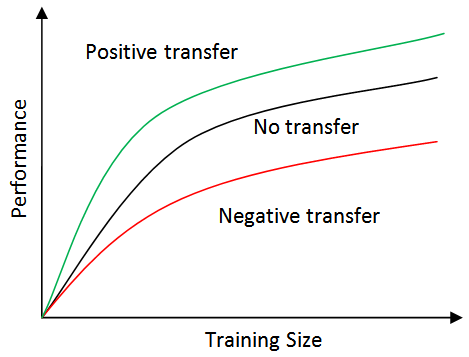
\includegraphics[scale=.5]{fig/negative.png}
\caption{Positive transfer VS Negative transfer. Relying on unrelated prior knowledge too much could lead to negative transfer.}\label{fig:neg}
\end{figure}
\begin{figure}
\centering
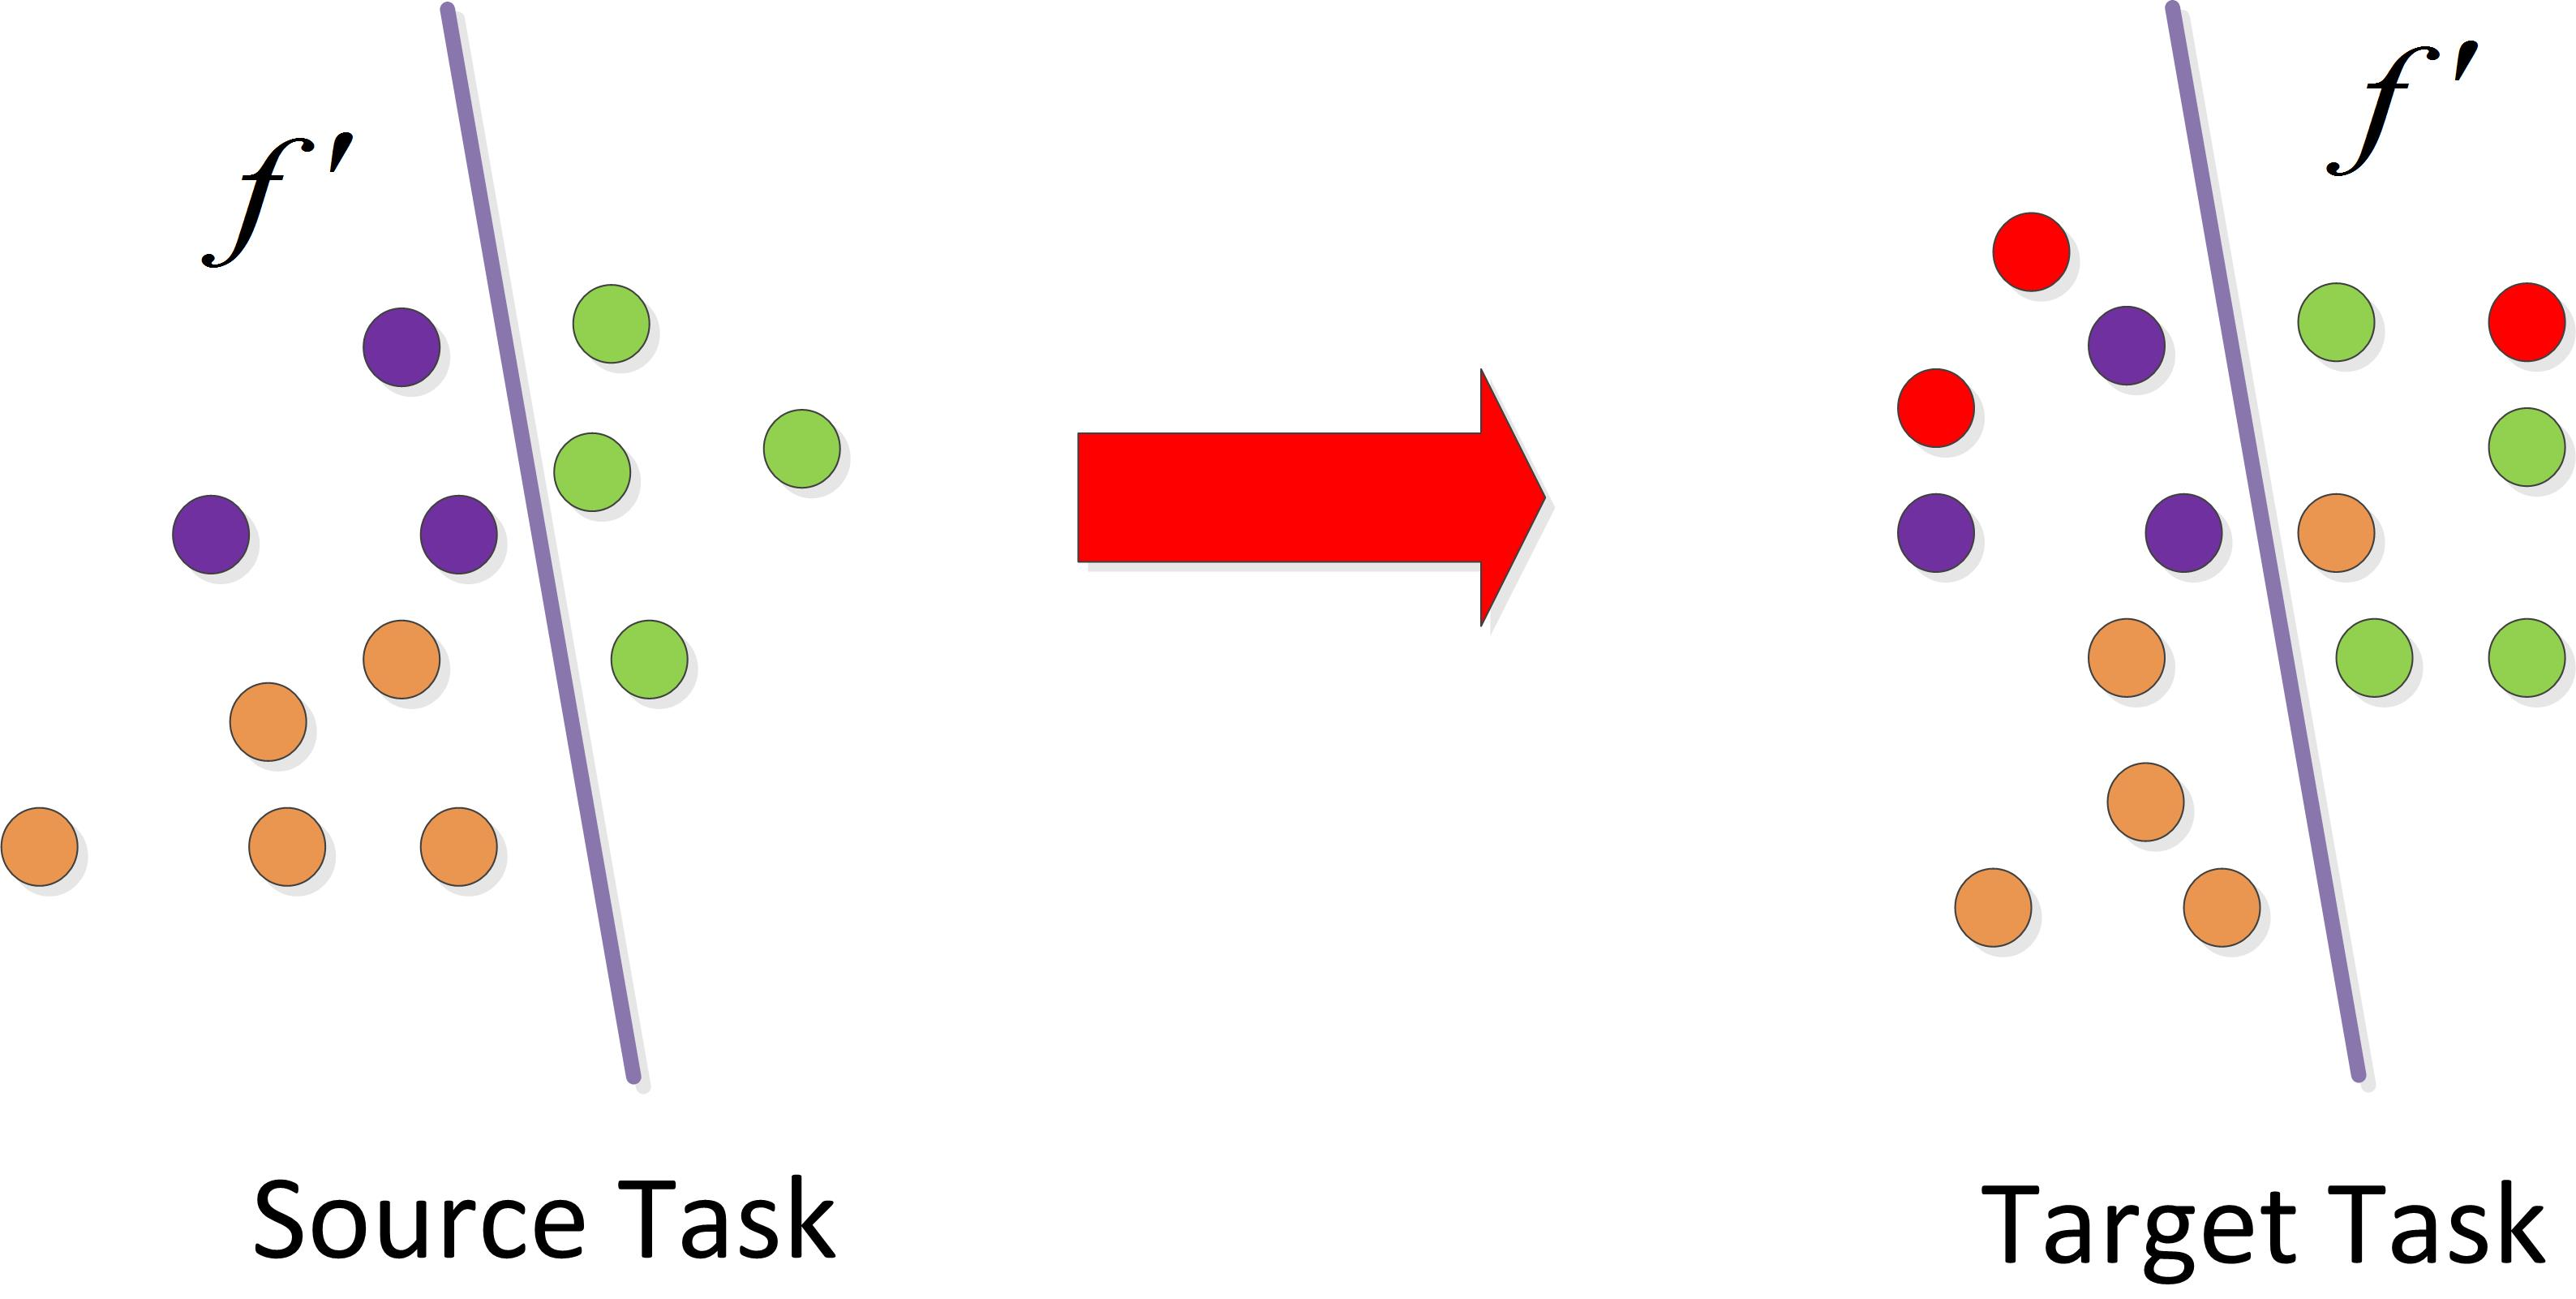
\includegraphics[scale=.4]{fig/domain.jpg}
\caption{Negative transfer happens when we transfer prior knowledge $f'$ to target one. Points with different color represent different categories. The data distribution would change even for identical categories in different task. The new added category (red points) can greatly affect the data distribution in target task. }\label{fig:distribution}
\end{figure}
In MITL, previous works focus on how to utilize the prior knowledge to preserve the performance for positive transfer rather than avoiding negative transfer. In our work, we focus on preventing negative transfer as well as preserving the performance for positive transfer. We propose our method, called Safety Multiclass Incremental Transfer Learning (SMITLe), that can both preserve the performance for positive transfer and avoid negative transfer. 
We use Least Square Support Vector Machine (LS-SVM) \cite{suykens1999least} as our basic model. The decision of each binary LS-SVM is the linear combination of the prior knowledge and empirical knowledge controlled by some transfer parameters. To measure the transferability of each prior knowledge, we estimate our transfer parameters using closed-form leave-one-out (LOO) error. Previous works theoretically suggest that closed-from LOO error can be an efficient way for parameter estimation with a small training set \cite{kuzborskij2013stability} \cite{cawley2006leave}. Then we propose our objective function that can balance the weight between the prior knowledge and empirical knowledge from target task. We also provide the theoretical proof that the transfer parameters optimized by our objective function can prevent negative transfer. Extensive empirical experiments show that other transfer learning baselines suffer from negative transfer while SMITLe can autonomously ignore the unrelated prior knowledge to prevent negative transfer. Then, we also show that when the prior knowledge is highly related to the target task (positive transfer), SMITLe can outperform the other transfer learning baselines by aggressively exploiting the prior knowledge.

The rest of this paper is organized as follow. We begin a brief review of the related work in Section \ref{sec:work}, including the goals and challenges of the transfer learning problems. In Section \ref{sec:prob}, we introduce the basic setting and some annotations of our problem. We provide the details of SMITLe, from parameter estimation to converge analysis and mathematical proof in Section \ref{sec:smitle}. In Section \ref{sec:exp}, we show the performance comparison between SMITLe and other baselines on a variety of experiments on AwA and Caltech datasets.
  


%\begin{figure}
%\centering
%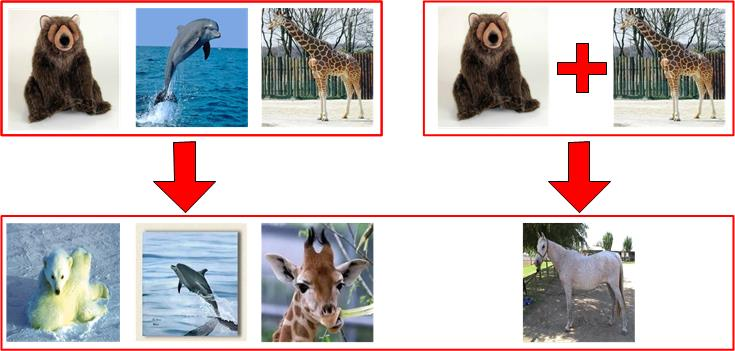
\includegraphics[scale=.4]{fig/transfer.jpg}
%\caption{}\label{fig:combine}
%\end{figure}

\section{Related Works}
The motivation of transfer knowledge between different domains is to apply the previous information from the source domain to the target one, assuming that there exists certain relationship, explicit or implicit, between the  feature space of these two domains \cite{pan2010survey}. Technically, previous work can be concluded into solving the following three issues: what, how and when to transfer \cite{tommasi2014learning}.


\textbf{What to transfer.} Previous work tried to answer this question from three different aspects: learning transferable instances, feature representations and model parameters. To utilize the data from previous classes, Lim et al. proposed a method of augmenting the training data by borrowing data from other classes for object detection \cite{lim2012transfer}. Learning transferable features means to learn common feature that can alleviate the bias of data distribution in target domain. Recently, Long et al. proposed a method that can learn transferable features with deep neural network  and showed some impressive results on some  benchmarks\cite{LongICML15}.Parameter transfer
approach assumes that the parameters of the model for the source task can be transfered to the target task. Yang et al. proposed Adaptive SVMs by transferring parameters from the auxiliary classifier from trained from source domain\cite{yang2007cross}. On top of Yang's work, Ayatar et al proposed PMT-SVM that can determine the transfer regularizer according to the target data automatically \cite{aytar2011tabula}. Tommasi et al. proposed Multi-KT that can utilize the parameters from multiple source models for the target classes  \cite{tommasi2014learning}.
Kuzborskij et al. proposed a similar method to learn new categories by leveraging over the known source \cite{kuzborskij2013n}.

\textbf{How to transfer.}


\section{Problem Statement}
Our method works in the following scenario. There is a image dataset (source data) containing $N$ categories and a classifier trained from this dataset to distinguish these $N$ categories. This (source) classifier and the features used to learn it is publicly accessible while the dataset itself is private (unknown distribution).  Now we collect our own image dataset (target data) coming from $N+1$ categories. This target dataset consists of $N$ identical categories to the source data and one new category related to the previous $N$ categories. In order to train a new classifier for our new task, we would expect our classifier to get better results with respect to 
\begin{itemize}
\item Maximize positive transfer. Since we know that these two task share some information, our classifier should transfer useful information as much as possible.
\item \hl{Minimize negative transfer. The data distribution of the source data is unknown. In the extreme situation, the data distribution of the two task could be totally different. Then these irrelevant prior knowledge should be considered as irrelevant and disposed.}
\end{itemize}

\hl{In this paper, we focus our work on transferring the knowledge with LS-SVM as the classifier for multi-class transfer problem. In the following we briefly introduce the mathermatical setting of our problem and show   }

\subsection{LS-SVM Setting and Definition}
Here we introduce the notations used in the rest of the paper. \hl{We use any letter with apostrophe to denote the information from the source data, e.g. if $f(x)$ denotes the model for the target task, $f'(x)$ denotes the model for the source one.}

% Table generated by Excel2LaTeX from sheet 'Sheet1'
\begin{table}[htbp]
  \centering
  \caption{useful notations in this paper}
    \begin{tabular}{|c|L{7cm}|}
    \hline
    $f'(x)$ & binary function for source task \\
    \hline
    $f(x)$  & binary function for target task \\
    \hline
    $\phi(x)$ &  function mapping the input sample into a high dimensional feature space. \\ \hline
    $K(x,x)$ & kernel matrix with  $\phi(x_i) \cdot\phi(x_j)$ corresponding to its element $(i,j)$\\ \hline
    $X$     & instance matrix with each row representing one instance \\\hline
    $W $    & (N+1)-column hyperplane matrix for target task. Each column represents one hyperplane of a binary model \\\hline
    $W'$    & hyperplane matrix for the source task \\\hline
    $a' $   & the Lagrangian multiplier matrix for source problem. Each column represents a set of  \\\hline
    $a $    & the Lagrangian multiplier matrix for target problem \\
    \hline
    $b',b$  & the bias vector for source and target task \\
        \hline
    $a_i,w_i$ & $i_{th}$ column of matrix $a$ and $w$\\\hline
    $d_\gamma$ &  diagonal matrix with$\left[ {{\gamma _1},...,{\gamma _N}} \right]$ in its main diagonal\\\hline
    $\beta$ & row vector $\left[ {{\beta _1},...,{\beta _N}} \right]$ to control the prior knowledge for the new category\\ \hline
    $\varepsilon_{ny_i}$&loss parameter. $\varepsilon _{n{y_i}}=1$ if $n=y_i$ and 0 otherwise\\ \hline
    \end{tabular}%
  \label{tab:notation}%
\end{table}%

 

Assume that, for our $(N+1)$-category target task, ${x} \in \mathcal{X}$ and ${y} \in \mathcal{Y}=\left\{1,2,...,N+1\right\}$ are the input vector and output for the learning task respectively. Meanwhile, we have a set of binary linear classifiers $f'_n(x)=\phi(x)w_n'+b_n'$, for $n=1,...,N$ trained from an unknown distribution with One-Versus-All (OVA) strategy.  Now we want to learn a set of new classifier $f_n(x)=\phi(x)w_n+b_n, n=1,...,N+1$, so that example $x$ is assigned to the category $j$ if $j \equiv \arg {\max _{n = 1,...,N+1}}\left\{{f_n}(x)\right\}$. In LS-SVM, the solution of the model parameters $(w_n,b_n)$ can be found by solving the following optimization problem:
\begin{equation*}
\begin{aligned}
\textbf{min} && R({w_n}) + \frac{C}{2}\sum\limits_i^l {({Y_{i,n}} - \phi ({x_i}){w_n} - {b_n})^2} \\
\end{aligned}
\end{equation*}
Where $R({w_n})$ is the regularization term to guarantee good generalization performance and avoid overfitting. $\mathbf{Y}$ is a encoded label matrix so that $Y_{in}=1$ if $y_i=n$ and $-1$ otherwise.  

In classic LS-SVM setting, the regularization term is set to $\frac{1}{2}\left\|w_n\right\|^2$ and the optimal $w_n=\phi(X)^T\alpha_n$ while the parameters $(\aleph_n,b_n)$ can be found by solving
\begin{equation}\label{eq:linear}
\left[ {\begin{array}{*{20}{c}}
{K(X,X) + \frac{1}{C}{\rm{I}}}&\mathbf{1}\\
\mathbf{1^T}&0
\end{array}} \right]\left( \begin{array}{l}
{\alpha _n}\\
{b_n}
\end{array} \right) = \left( \begin{array}{l}
{Y_n}\\
0
\end{array} \right)  
\end{equation}
Here $I$ is the identity matrix and $\mathbf{1}$ is a column vector with all its elements equal to 1.

Now our task can be divided into two separate part: learning the $N$ overlapped categories and the new category. 
\hl{We know that the source and target share $N$ categories.} From previous work \cite{yang2007cross}, the regularization term can be written as $\frac{1}{2}{{{\left\| {{w_n} - {\gamma _n}{{w'}_n}} \right\|}^2}}$. Here, $\gamma_n$ is the regularization parameter controlling the amount of transfer.
\hl{For the task for new category}, we can use multi-source kernel learning strategy in \cite{tommasi2014learning} 


So the multi-class transfer problem can be solved by optimizing the following objective function:
\begin{equation}\label{eq:opt}
\begin{aligned}
\textbf{min}\qquad {} & \frac{1}{2}\sum\limits_{n = 1}^N {{{\left\| {{w_n} - {\gamma _n}{{w'}_n}} \right\|}^2}}  + \frac{1}{2}{\left\| {{w_{N + 1}} - \sum\limits_{k = 1}^N {w{'_k}{\beta _k}} } \right\|^2}\\& \frac{C}{2}\sum\limits_{n = 1}^{N + 1} {\sum\limits_{i = 1}^l {e_{i,n}^2} }  \\
\textbf{s.t.}\qquad {} &{e_{i,n}} = {Y_{i,n}} - \phi ({x_i}){w_n} - {b_n}
\end{aligned}
\end{equation}

The closed-form of the optimal solution to  Eq. (\ref{eq:opt}) is:
\begin{equation*}
\begin{array}{*{20}{c}}
{{w_n} = {\gamma _n}{{w'}_n} + \sum\limits_i^l {{\alpha _{in}}{\phi(x_i)}} }&{n = 1,...,N}\\
{{w_{N + 1}} = \sum\limits_k^N {{\beta _k}{{w'}_k}}  + \sum\limits_i^l {{\alpha _{i(N + 1)}}{\phi(x_i)}} }&{}
\end{array}
\end{equation*}
Here $\alpha_{ij}$ is the element $(i,j)$ in $\boldsymbol{\alpha}$. The intuitive interpretation of the results above is that the hyperplane of the target problem is the linear combination of the prior knowledge (first part of the right side) and empirical knowledge from target task (second part of the right side).

Let $\psi$ denotes the first term of left-hand side in Eq. (\ref{eq:linear}) and let:
\begin{equation}
\begin{array}{c}
 {\psi}\left[ {\begin{array}{*{20}{c}}
{\boldsymbol{\alpha} '}\\
{\boldsymbol{b}'}
\end{array}} \right] = \left[ {\begin{array}{*{20}{c}}
Y\\
0
\end{array}} \right]\\
{\psi}\left[ {\begin{array}{*{20}{c}}
{\boldsymbol{\alpha} ''}\\
{\boldsymbol{b}''}
\end{array}} \right] = \left[ {\begin{array}{*{20}{c}}
{X{{\left( {W'} \right)}^T}}\\
0
\end{array}} \right]
\end{array}
\end{equation}
We have:
\begin{equation}\label{eq:solution}
 \boldsymbol{\alpha}  = \boldsymbol{\alpha} ' - \left[ {\begin{array}{*{20}{c}}
 {\boldsymbol{\alpha} ''{d_r}}&{{\boldsymbol{\alpha} ''\boldsymbol{\beta ^T}}}
 \end{array}} \right]
\end{equation}
From Eq. (\ref{eq:solution}) we can see that, the solution of Eq. (\ref{eq:linear}) is completed once $\boldsymbol{\gamma}=\left[ \gamma_1,...,\gamma_N\right] $ and $\boldsymbol{\beta}$ are set.

\subsection{Optimize $\gamma$ and $\beta$}
\hl{introduce LOO error estimation. In this part, we introduce our method to estimate proper $\boldsymbol{\gamma}$ and $\boldsymbol{\beta}$ that can prevent negative transfer.}
From above, we can see that the hyperplane for the target problem is determined by $\boldsymbol{\gamma}$ and $\boldsymbol{\beta}$. Negative transfer happens when the model aggressively leverage over irrelevant prior knowledge, i.e. set a  large value to $\boldsymbol{\gamma}$ and $\boldsymbol{\beta}$. However, aggressive leverage over informative priors can improve the performance of the transfer model greatly. Inspired by some previous works \cite{tommasi2014learning} \cite{kuzborskij2013n}, we proposed \hl{our method} that can minimize the affect of negative transfer from irrelevant priors.

\hl{As we mentioned above, another important advantage of LS-SVM over the other model is that we can get unbiased LOO error in closed form} \cite{cawley2006leave}. The unbiased LOO estimation for sample $x_i$ can be written as:
\begin{equation}
{\hat Y_{i,n}} = {Y_{i,n}} - \frac{{{\alpha _{in}}}}{{\psi_{ii}^{ - 1}}}{\text{    for   }}n = 1,...,N + 1
\end{equation}
Here $\psi^{-1}$ is the inverse of matrix $\psi$ and  $\psi_{ii}^{-1}$ is its $ith$ diagonal element. 

\hl{Let us call $\xi_i$ the empirical error of our multi-class prediction for example $x_i$, and $\xi_i$ can be defined as} \cite{crammer2002algorithmic}:
\begin{equation}\label{eq:train_loss}
\xi_i(\gamma,\beta) = \mathop {\max }\limits_{n \in \left\lbrace 1,...,N+1 \right\rbrace } {\left[ {1 - {\varepsilon _{n{y_i}}} + {{\hat Y}_{in}}\left( {\gamma ,\beta } \right) - {{\hat Y}_{i{y_i}}}\left( {\gamma ,\beta } \right)} \right]}
\end{equation}
Where $\varepsilon _{n{y_i}}=1$ if $n=y_i$ and 0 otherwise. $\xi_i(\gamma,\beta)>0$ if example $x_i$ is misclassified. The intuition behind this loss function is to enforce the distance between the true class and other classes to be at least 1.

Then we define our objective function as:
\begin{equation}\label{loss}
\begin{aligned}
& \textbf{min}
& & \frac{{{\lambda _1}}}{2}\sum\limits_{n = 1}^N {{{\left\| {{\gamma _n}} \right\|}^2}}  + \frac{{{\lambda _2}}}{2}\sum\limits_{n = 1}^N {{{\left\| {{\beta _n}} \right\|}^2}}  + \sum\limits_{i = 1}^l {{\xi _i}}   \\
& \textbf{s.t.}
& & 1 - {\varepsilon _{n{y_i}}} + {\hat Y_{in}}\left( {\gamma ,\beta } \right) - {\hat Y_{i{y_i}}}\left( {\gamma ,\beta } \right) \le {\xi_i};\\
& & &\lambda_1,\lambda_2 \ge 0
\end{aligned}
\end{equation}

Here $\lambda_1$ and $\lambda_2$ are two regularization parameters to prevent overfitting. 
From the objective function above we can see that, for certain $\lambda_1$ and $\lambda_2$, when the prior knowledge is unrelated and negative transfer happens, increasing $\boldsymbol{\gamma}$ and $\boldsymbol{\beta}$ leads to larger punishment from both regularization and empirical error from target task. Decreasing the affect of prior knowledge reduces the loss of the objective function and eventually prevents negative transfer. Moreover, we also prove that this objective function can avoid negative transfer (for more details, see Theorem \ref{th:1}). On the other hand, if the prior knowledge is related, even though, increasing $\boldsymbol{\gamma}$ and $\boldsymbol{\beta}$ leads to larger punishment, it also leads to smaller empirical error on the target problem. So the algorithm compromises between the prior and empirical knowledge. \hl{Besides, there are some other properties that make our method efficient.}(see Section \ref{subsec:analysis})


By adding a dual set of variables, one for each constraint, we get the Lagrangian of the optimization problem:
\begin{equation}\label{eq:dual}
\begin{aligned}
 \textbf{max}\qquad {}& L\left( {\gamma ,\beta ,\xi ,\eta } \right) =\\
 &\frac{{{\lambda _1}}}{2}\sum\limits_{n = 1}^N {{{\left\| {{\gamma _n}} \right\|}^2}}  + \frac{{{\lambda _2}}}{2}\sum\limits_{n = 1}^N {{{\left\| {{\beta _n}} \right\|}^2}}  + \sum\limits_{i = 1}^l {{\xi _i}} \\
   &+ \sum\limits_{i,n} {{\eta _{i,n}}\left[ {1 - {\varepsilon _{n{y_i}}} + {{\hat Y}_{in}}\left( {\gamma ,\beta } \right) - {{\hat Y}_{i{y_i}}}\left( {\gamma ,\beta } \right) - {\xi _i}} \right]}  \\
 \textbf{s.t.} \qquad {} & \forall i,n \quad {} {\eta _{i,n}} \ge 0
\end{aligned}
\end{equation}

The problem of Eq. \eqref{eq:dual} is a non-differentiable strongly convex problem. The sub-gradient of it can be written as:
\begin{equation*}
{\Delta _\gamma }=\begin{cases}
\boldsymbol{0}&{y_i}=n\\
\left[ {0,..,\frac{{\alpha ''}_{in}}{\psi _{ii}^{ - 1}},.., - \frac{{\alpha ''}_{i{y_i}}}{\psi _{ii}^{ - 1}},..,0} \right]&{y_i},n = 1,...N\\
\left[ {0,..,\frac{{\alpha ''}_{in}}{\psi _{ii}^{ - 1}},..,0} \right]&{y_i} = N + 1;n = 1,...N\\
\left[ {0,.., - \frac{{\alpha ''}_{i{y_i}}}{\psi _{ii}^{ - 1}},..,0} \right]&\text{otherwise}
\end{cases}
\end{equation*}
\begin{equation*}
{\Delta _\beta }=\begin{cases}
 - \sum {{{\alpha ''}_{ik}}{\beta _k}} &{y_i} = N + 1;n = 1,...N\\
 \sum {{{\alpha ''}_{ik}}{\beta _k}} &{y_i} = 1,..N;n = N+1\\
\boldsymbol{0}&\text{otherwise}\\
\end{cases}
\end{equation*}
To obtain the optimal values for the problem above, we introduce our method \hl{using sub-gradient descent }\cite{BoydCO} and summarize it in Alg. \ref{alg:1}. 
\begin{algorithm}
       \caption{$\gamma$ optimization}\label{alg:1}
        \begin{algorithmic}[1]
            \REQUIRE $\psi,\alpha',\alpha'',T,\psi$,
            \ENSURE $\gamma=\left\{\gamma^1,...,\gamma^n\right\}, \beta$
            \STATE $\beta \leftarrow 0, \gamma \leftarrow 1$
            \FOR {$iter=1$ to $T$}
                \STATE $\hat Y \leftarrow Y - {\left( {\psi \circ I} \right)^{ - 1}}\left( {\alpha' - \left[ {\begin{array}{*{20}{c}}
{\alpha''d_\gamma }&{\alpha''\beta^T }
\end{array}} \right]} \right)$
                \STATE ${\Delta _\gamma }=0, {\Delta _\beta }=0$
                \FOR {$i=1$ to $l$}
                	\STATE ${\Delta _\gamma }\leftarrow {\Delta _\gamma }+\lambda_1\gamma$ 
                	\STATE ${\Delta _\beta }\leftarrow {\Delta _\beta }+\lambda_2\beta$
                	\FOR {$r=1$ to $N+1$}
	                    \STATE $l_{ir} = 1 - {\varepsilon _{{y_i}r}} + {\hat Y_{ir}} - {\hat Y_{i{y_i}}}$
	                    \IF{$l_{ir}>0$}
	                        \IF {$y_i,r \in \{1,...,N\}$}
	                            \STATE $\Delta _\gamma^{{y_i}} \leftarrow \Delta _\gamma^{{y_i}} - \frac{{{\alpha''_{i{y_i}}}}}{{{\psi^{-1}_{ii}}}}$%
	                            \STATE $\Delta _\gamma^{{r}} \leftarrow \Delta _\gamma^{{r}} + \frac{{{\alpha''_{i{r}}}}}{{{\psi^{-1}_{ii}}}}$%
	                        \ELSIF {$y_i=N+1$}
	                            \STATE ${\Delta _\beta } \leftarrow {\Delta _\beta } - \frac{{{\alpha''_i}}}{{{\psi^{-1}_{ii}}}}$
	                             \STATE $\Delta _\gamma^{{r}} \leftarrow \Delta _\gamma^{{r}} + \frac{{{\alpha''_{i{r}}}}}{{{\psi^{-1}_{ii}}}}$%
	                        \ELSE
	                            \STATE $\Delta _\gamma^{{y_i}} \leftarrow \Delta _\gamma^{{y_i}} - \frac{{{\alpha''_{i{y_i}}}}}{{{\psi^{-1}_{ii}}}}$
	                             \STATE        ${\Delta _\beta } \leftarrow {\Delta _\beta } + \frac{{{\alpha''_i}}}{{{\psi^{-1}_{ii}}}}$
	                        \ENDIF
	                    \ENDIF
	                 \ENDFOR %class ends   
                \ENDFOR %examples ends
                \STATE $\beta \leftarrow \beta - \frac{{{\Delta _\beta }}}{{l \times {iter} }}$
                \STATE $\gamma  \leftarrow \gamma  - \frac{{{\Delta _\gamma }}}{{l\times {iter} }}$
             \ENDFOR %iteration ends
        \end{algorithmic}
\end{algorithm}

\subsection{Analysis}\label{subsec:analysis}
\hl{In this part, we mainly discuss our method in two aspects: convergence analysis and mathermatical proof of preventing negative transfer.} 

\hl{Convergence analysis}
The primal problem \eqref{loss} becomes the strongly convex problem by adding the L2 regularization terms. Optimizing the strongly convex problem can lead to the following error bound:
%\begin{lemma}[Converge lemma]
%Let $f(\mu)$ be a 1-strongly convex function. Let $\mu_1,...,\mu_t$ be a sequence corresponding to $\mu_t=(\sqrt{\lambda_1}\gamma^t,\sqrt{\lambda_2}\beta^t)$. Let $\Delta_t$ be the sub-gradient for $f(\mu_t)$ and $\mu^*=(\sqrt{\lambda_1}\gamma^*,\sqrt{\lambda_2}\beta^*)$
%\end{lemma}

Let $\mu_1,...,\mu_t$ be a sequence corresponding to $\mu_t=(\sqrt{\lambda_1}\gamma^t,\sqrt{\lambda_2}\beta^t)$. Problem \eqref{eq:loss} can be rewritten as:
\begin{equation*}
J(\mu)=\frac{1}{2}{\left\| \mu  \right\|^2} + \sum\limits_{i = 1}^l {{\xi _i}\left( \mu  \right)} 
\end{equation*}
Let $\Delta_t$ be the sub-gradient for $J(\mu_t)$ and  $\mu^*=(\sqrt{\lambda_1}\gamma^*, \sqrt{\lambda_2}\beta^*)$ be the optimal solution for it. Assume that $\left\| {{\Delta _t}} \right\| \le G$. According to Lemma 1 in \cite{shalev2011pegasos}, we have:
\begin{equation}
J({\mu_t}) - J(\mu^*) \le \frac{{{G^2}}}{{2t}}\left( {1 + \ln \left( t \right)} \right)
\end{equation}
This means that SMITLe converges at the rate of $O(\frac{\log(t)}{t})$.



\hl{Superior bound analysis}
\begin{theorem}\label{th:1}
Assume that $\bar \xi_i$ is the multi-class loss of example $x_i$ when $\gamma=\beta = \mathbf{0}$. Let $\gamma^*, \beta^*$ be the optimal solution for Eq. \eqref{eq:dual} and $\xi_i^*$ be the multi-class loss with respective to example $x_i$. Then for every example $x_i \in \mathcal{X}$, we have:\[\sum\limits_i {{\xi _i}}  \le \sum\limits_i {{{\bar \xi }_i}} \]
\end{theorem}
\begin{proof}
For simplification, let $\delta_i=1$ if $i=N+1$ and 0 otherwise, and  ${\theta _{ij}} = {\alpha ''_{ij}}\left( {1 - {\delta _j}} \right)/\psi_{ii}^{ - 1}$. Eq. \eqref{eq:train_loss} can be written as:
\begin{equation}\label{eq:loss_simple}
\begin{split}
{\xi _i}(\gamma ,\beta )=&\mathop {\max }\limits_{n} \bigg \{ {\varepsilon _{n{y_i}}} - 1 + \frac{{\left( {{{\alpha '}_{i{y_i}}} - {{\alpha '}_{in}}} \right)}}{{\psi _{ii}^{ - 1}}} + {\theta _{in}}{\gamma _n} \\
&- {\theta _{i{y_i}}}{\gamma _{{y_i}}} + \left( {{\delta _n} - {\delta _{{y_i}}}} \right)\sum\limits_k {\frac{{{{\alpha ''}_{ik}}{\beta _k}}}{{\psi_{ii}^{ - 1}}}}  \bigg\}
\end{split}
\end{equation}
When $\mathbf{\gamma}=\mathbf{\beta} = \mathbf{0}$, from Eq. \eqref{eq:loss_simple} we can get:
\begin{equation*}
{\bar \xi _i} = \mathop {\max }\limits_n \left[ { {\varepsilon _{n{y_i}}}-1 + \frac{{\left( {{{\alpha '}_{i{y_i}}} - {{\alpha '}_{in}}} \right)}}{{\psi _{ii}^{ - 1}}}} \right]
\end{equation*}
To obtain the optimal value of $\gamma$ and $\beta$, we have to seek the saddle point of the Lagrangian problem in \eqref{eq:dual} by finding the minimum for the prime variables $\left\{ \gamma, \beta, \xi \right\}$ and the maximum for the dual variables $\eta $. To find the minimum of the primal problem, we require:
\begin{equation*}
\frac{{\partial L}}{{\partial {\xi _i}}} = 1 - \sum\limits_n {{\eta _{in}}}  = 0 \to \sum\limits_n {{\eta _{in}}}  = 1
\end{equation*}   
Similarly, for $\gamma$ and $\beta$, we require:
\begin{eqnarray}\label{eq:opt_gama}
\frac{{\partial L}}{{\partial {\gamma _n}}} &=& {\lambda _1}{\gamma _n} + \sum\limits_i {{\eta _{in}}{\theta _{in}}}  - \sum\limits_{i,n = {y_i}} {\left( {\sum\limits_q {{\eta _{iq}}} } \right){\theta _{in}}{\gamma _n}}  \nonumber\\
&=_1 &{\lambda _1}{\gamma _n} + \sum\limits_i {{\eta _{in}}{\theta _{in}}}  - \sum\limits_i {{\varepsilon _{n{y_i}}}{\theta _{in}}}  = 0  \nonumber\\
&\Rightarrow & \gamma _n^* = \frac{1}{{{\lambda _1}}}\sum\limits_i {\left( {{\varepsilon _{n{y_i}}} - {\eta _{in}}} \right){\theta _{in}}} 
\end{eqnarray}
In $=_1$ we use the facts that $\sum_n\eta_{in}=1$ and use $\varepsilon_{ny_i}$ to replace it.
\begin{eqnarray}\label{eq:opt_beta}
\frac{{\partial L}}{{\partial {\beta _n}}} &=& {\lambda _2}{\beta _n} + \left[ {\sum\limits_{i,n} {\frac{{{\eta _{in}}{{\alpha ''}_{in}}}}{{\psi_{ii}^{ - 1}}}\left( {{\delta _n} - {\delta _{{y_i}}}} \right)} } \right] = 0 \nonumber \\
&\Rightarrow &\beta _n^* = \frac{1}{{{\lambda _2}}}\sum\limits_{i,n} {\frac{{{\eta _{in}}{{\alpha ''}_{in}}}}{{\psi _{ii}^{ - 1}}}\left( {{\delta _{{y_i}}} - {\delta _n}} \right)} 
\end{eqnarray}
As the strong duality holds,the primal and dual objectives coincide. Plug Eq \eqref{eq:opt_gama} and \eqref{eq:opt_beta} into Eq. \eqref{eq:dual}, we have:
\begin{equation*}
\sum\limits_{i,n} {{\eta _{in}}\left[ {1 - {\varepsilon _{n{y_i}}} + {{\hat Y}_{in}}\left( {\gamma^* ,\beta^* } \right) - {{\hat Y}_{i{y_i}}}\left( {\gamma^* ,\beta^* } \right) - {\xi _i^*}} \right]}=0
\end{equation*}
Expand the equation above, we have:
\begin{eqnarray}\nonumber
\sum\limits_{i,n} {{\eta _{in}}\left[ { {\varepsilon _{n,{y_i}}}-1 + \frac{{\left( {{{\alpha '}_{i{y_i}}} - {{\alpha '}_{in}}} \right)}}{{\psi_{ii}^{ - 1}}} - {\xi _i}} \right]} \nonumber\\ 
= {\lambda _1}\sum\limits_r {{{\left\| {\gamma _r^*} \right\|}^2}}  + {\lambda _2}\sum\limits_r {{{\left\| {\beta _r^*} \right\|}^2}}  \ge 0\nonumber
\end{eqnarray}
Rearranging the above, we obtain:
\begin{eqnarray}\label{eq:link1}
\sum\limits_{i,n} {{\eta _{in}}\left[ { {\varepsilon _{n,{y_i}}} -1+ \frac{{\left( {{{\alpha '}_{i{y_i}}} - {{\alpha '}_{in}}} \right)}}{{\psi_{ii}^{ - 1}}}} \right]} \nonumber\\ 
 \ge \sum\limits_{i,n} {{\eta _{in}}{\xi _i}}  = \sum\limits_i {{\xi _i}} 
\end{eqnarray}
The left-hand side of Inequation \eqref{eq:link1} can be bounded by:
\begin{eqnarray}
&&\sum\limits_{i,n} {{\eta _{in}}\left[ { {\varepsilon _{n{y_i}}}-1 + \frac{{\left( {{{\alpha '}_{i{y_i}}} - {{\alpha '}_{in}}} \right)}}{{\psi_{ii}^{ - 1}}}} \right]} \nonumber\\ &&\le \sum\limits_i {\left( {\sum\limits_n {{\eta _{in}}\mathop {\max }\limits_r \left\{ { {\varepsilon _{r{y_i}}} -1 + \frac{{\left( {{{\alpha '}_{i{y_i}}} - {{\alpha '}_{ir}}} \right)}}{{\psi_{ii}^{ - 1}}}} \right\}} } \right)}  \nonumber\\
&&= \sum\limits_i {\left( {\sum\limits_n {{\eta _{in}}{{\bar \xi }_i}} } \right)}  = \sum\limits_i {\bar \xi_i }
\end{eqnarray}
\end{proof}

When setting $\gamma=\beta = \mathbf{0}$, we don't utilize any knowledge from previous task (see Eq. \eqref{eq:opt}). From Theorem \ref{th:1} we can conclude \hl{our method can always outperform the method learning directly.}

\hl{discuss $\lambda$}

\section{Experiment}
In this section, we show empirical results of our algorithm on different transferring situations on two datasets: AwA\footnote{The features of AwA dataset is available from http://attributes.kyb.tuebingen.mpg.de/} \cite{lampert2009learning} and Caltech-256\footnote{Images for Caltech-256 is available from http://www.vision.caltech.edu/Image\_Datasets/Caltech256/} \cite{griffin2007caltech}. We design the following \hl{3 sets of experiments: learning from informative prior, irrelevant prior and mixed prior, } to show the effectiveness of our algorithm.
\subsection{Dataset \& Settings}
Caltch-256 contains 30607 images from 256 categories. We select the following 10 categories: \textit{bat, bear, dolphin, giraffe, gorilla, horse, leopard, raccoon, skunk, zebra} as our dataset.

AwA dataset consists of 50 animal categories. Its source images is not publicly accessible and we can only access the six pre-extracted feature representations for each image. This property makes it natural as the unknown distribution source dataset to train the prior knowledge. We choose the identical 10 categories as those in Caltech-256 as the source dataset.

\subsection{Baselines}
We compare our algorithm with two kinds of baselines. The first one is methods without leveraging any prior knowledge (no transfer baselines). The second consists of some methods with transfer techniques. Here are the no transfer baselines. 

\textbf{0+T(arget):} LS-SVM trained only on target data. This baseline can be the indicator as the best performance in the \hl{bad oracle experiment.}

\textbf{S(ource)+T(arget):} \hl{This baseline is only used in good oracle experiment.} We combined the source and target data, assuming that we have fully access to all data, to train the LS-SVM. The result of this baseline might be considered as the best performance achieved in the experiment as well as an important reference for assessing the models with transfer learning methods.

\textbf{S(ource)+1:} This method only train a new binary LS-SVM for the new category. For the rest of the classes, we use the predictions of the classifiers trained from source data directly. This is arguably the easiest way for transfer learning. \hl{In some of our experiments, it is a good indicator when negative transfer happens.} 

We select the following 3 methods as our transfer baselines. The general property of these 3 methods is that they all try to leverage multiple prior knowledge to benefit the transfer procedure.

\textbf{MKTL \cite{jie2011multiclass}:} This method uses the output of prior models as extra feature inputs, and automatically determine from which prior models to transfer and how much to transfer.


\textbf{Multi-KT \cite{tommasi2014learning}:} This method has similar idea with MKTL. It uses LOO error to determine how much to transfer from prior models and convert it into solving the convex optimization problem.

\textbf{MULTIpLE \cite{kuzborskij2013n}:} The basic setting of this method is similar like ours. It is designed to balance the performance between learning the new category and preserving the model from prior knowledge.

\subsection{transfer from good oracle}
\begin{figure*}
\centering

\subfloat[Results on Caltech dataset ]{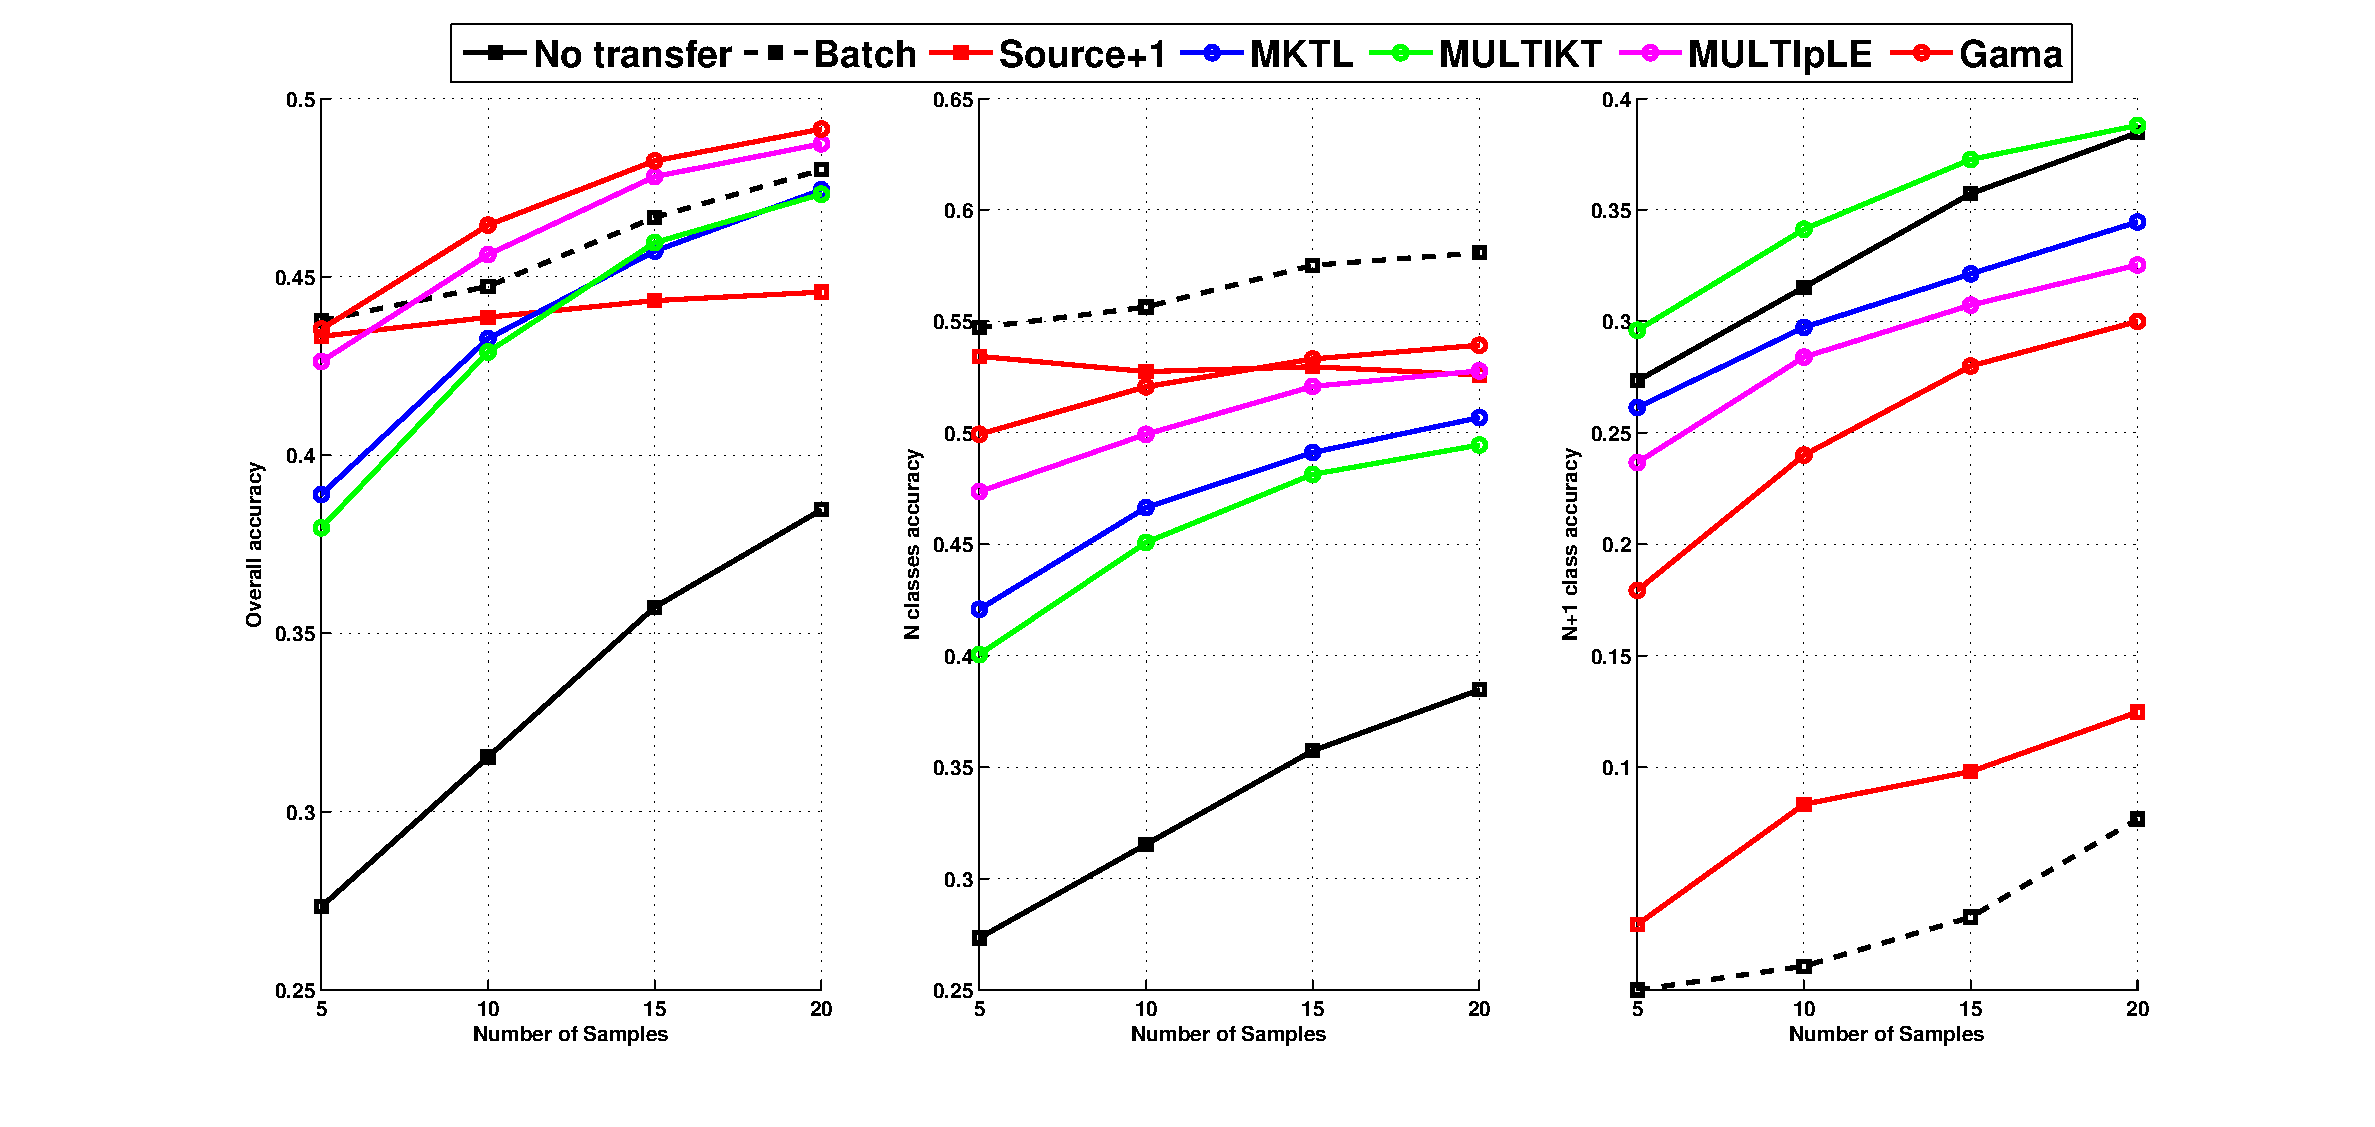
\includegraphics[width=\textwidth,height=5cm]{fig/C2C_RBF.eps}}
\newline
\subfloat[Results on AwA dataset] {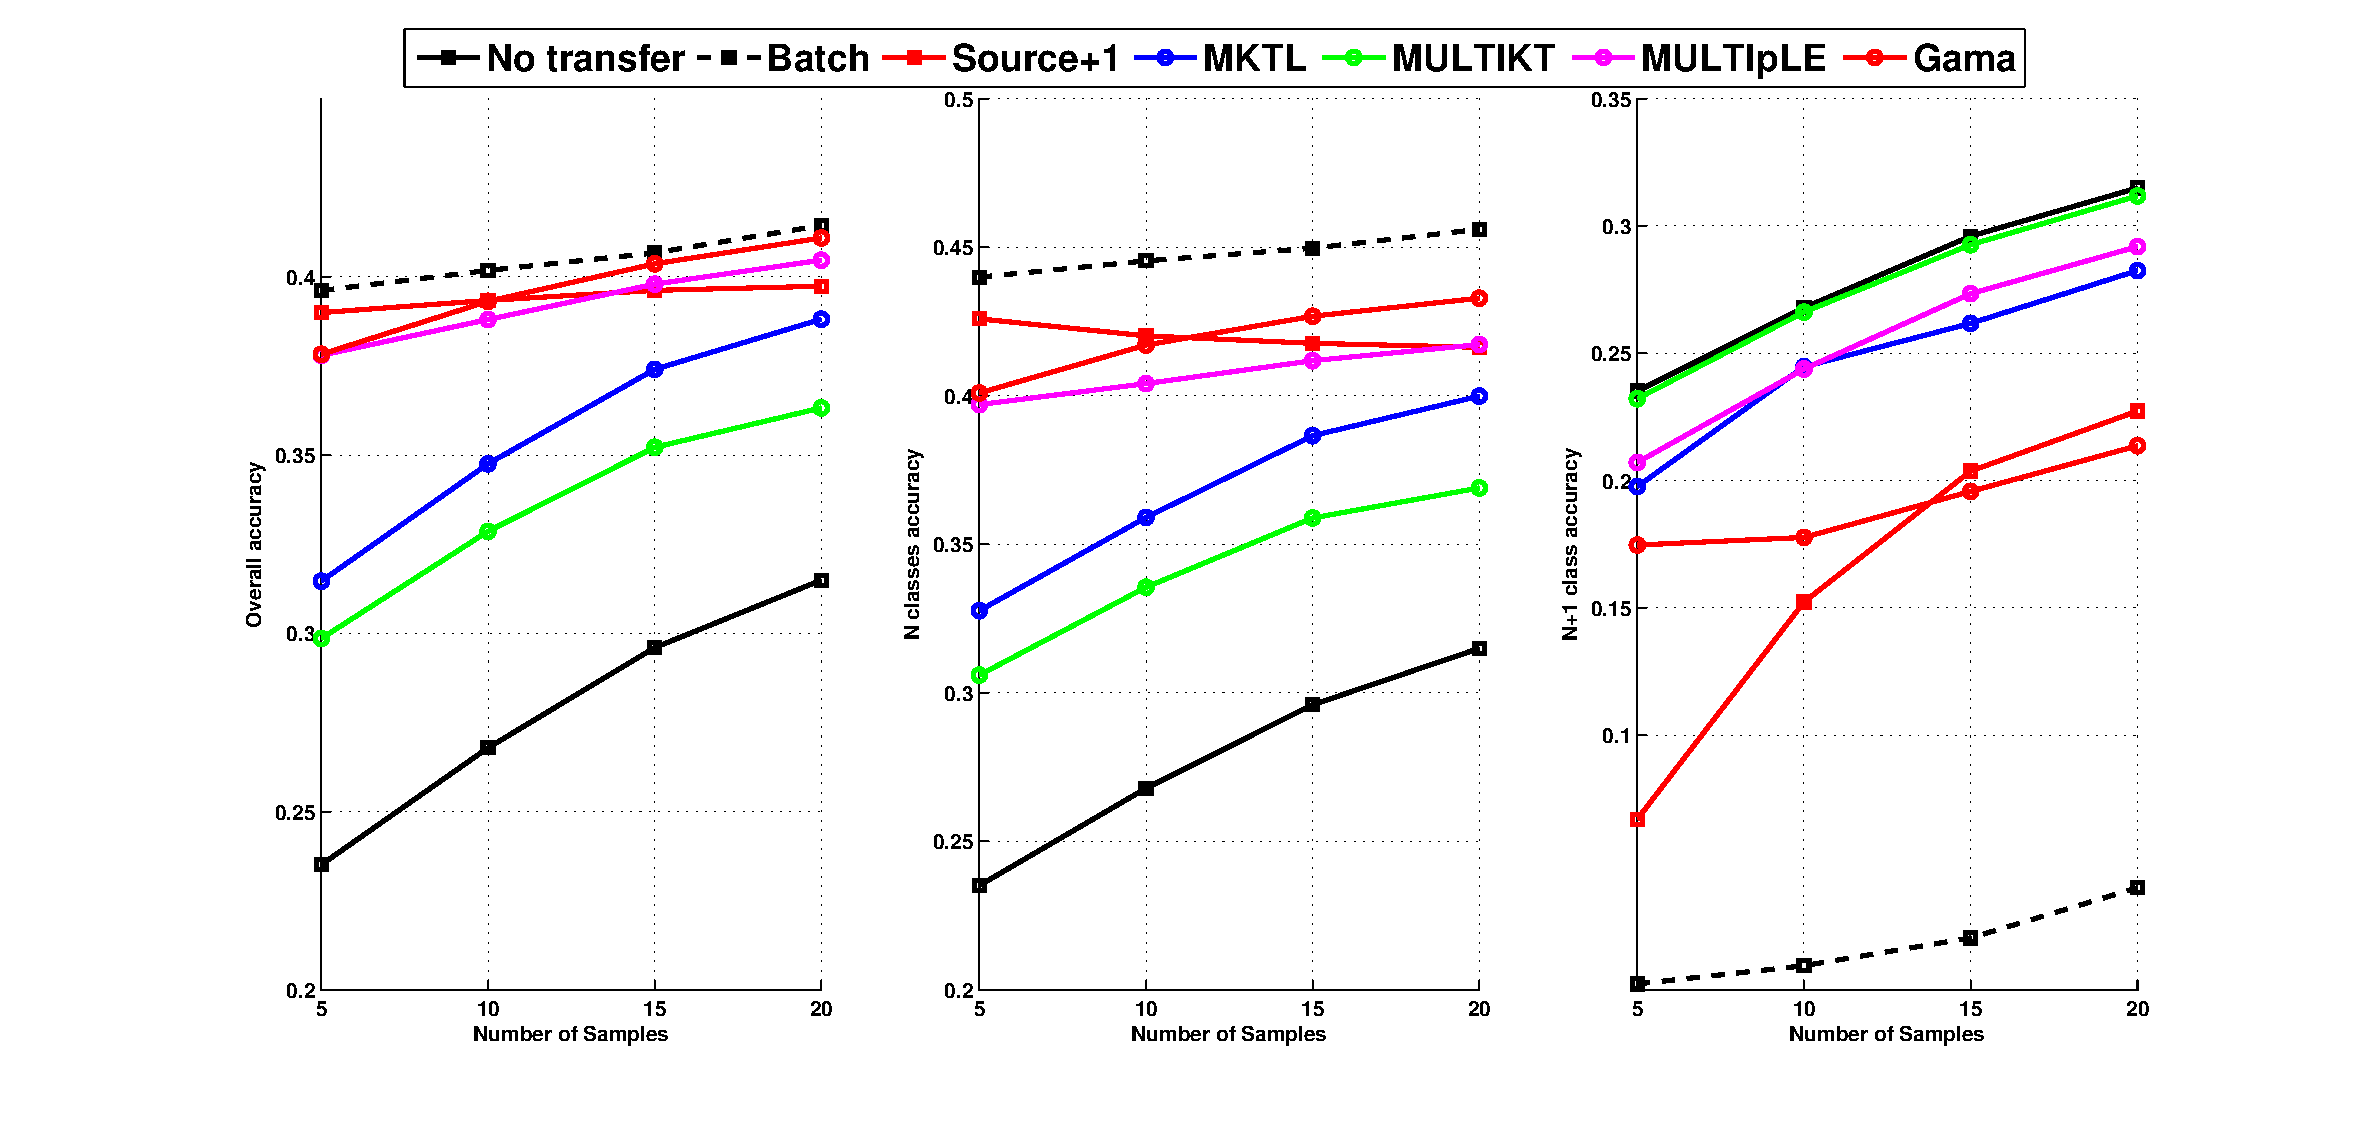
\includegraphics[width=\textwidth,height=5cm]{fig/A2A_RBF.eps}}

\caption{Acc for good oracle}
\end{figure*}

\subsection{from bad oracle}
\begin{figure*}
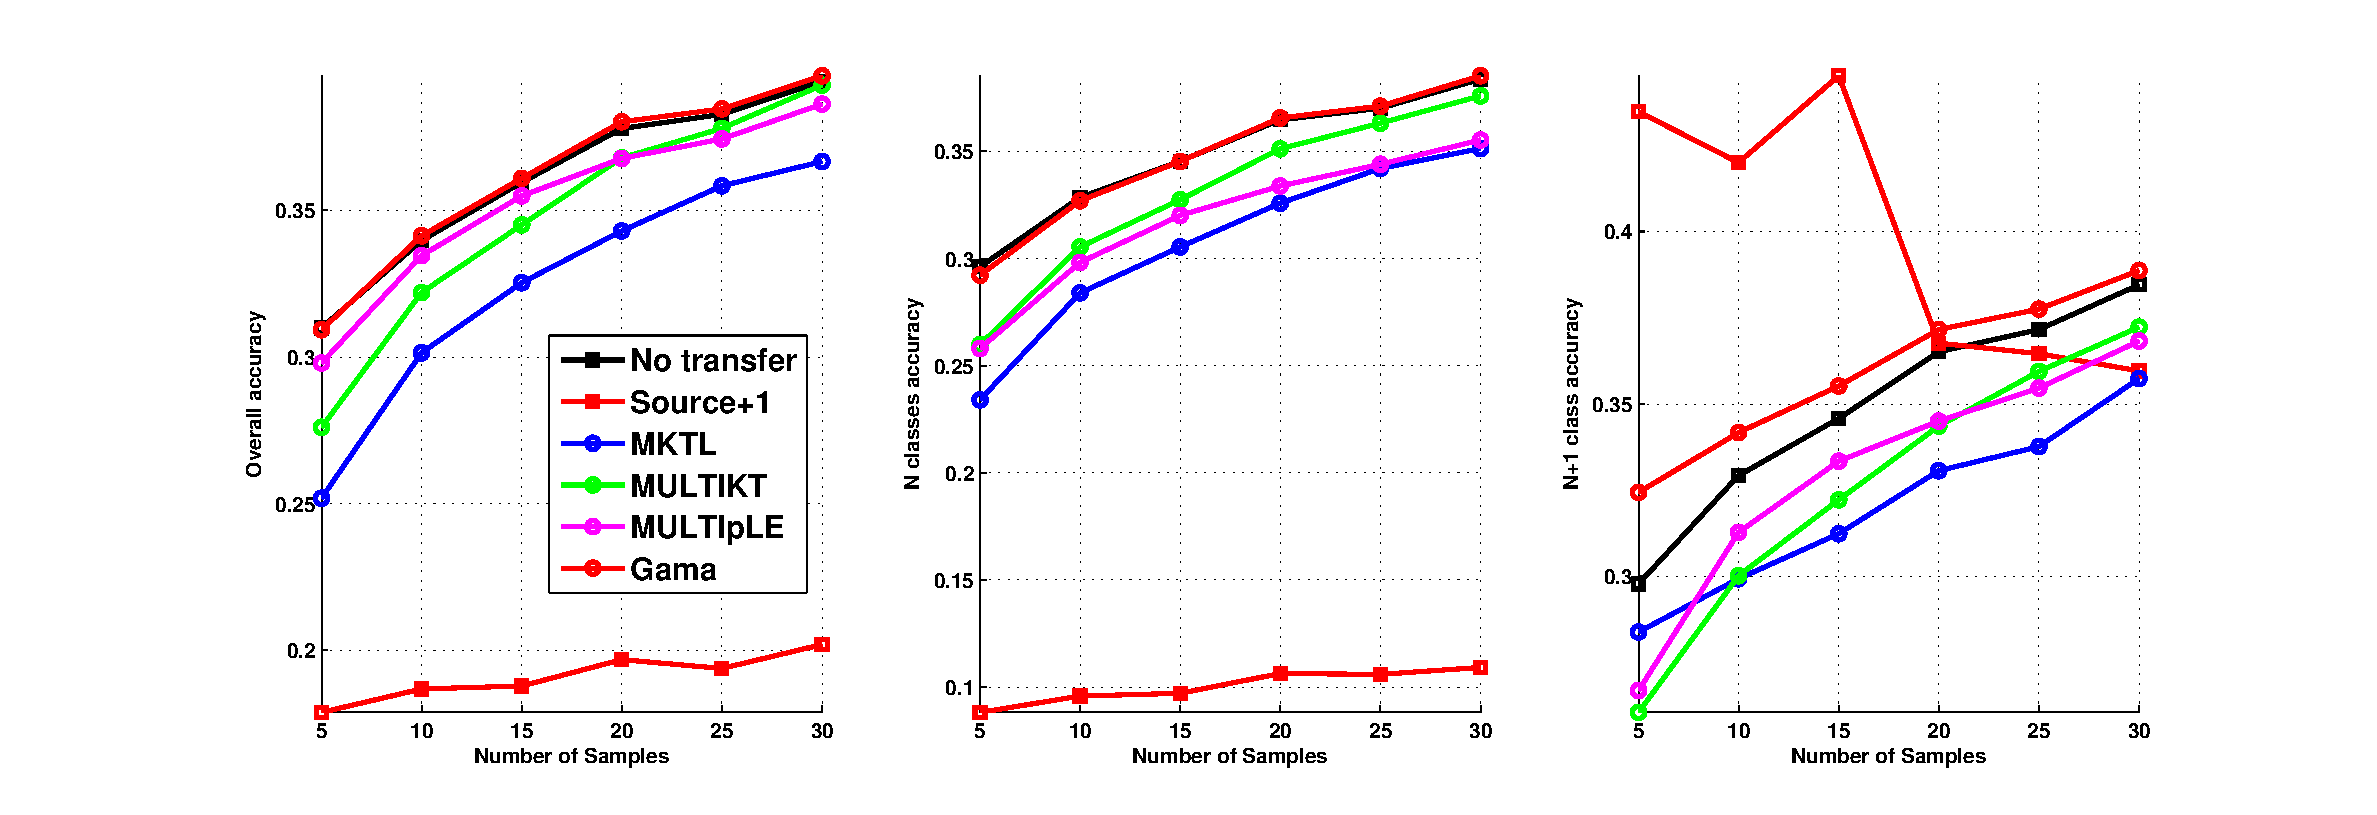
\includegraphics[width=\textwidth,height=5cm]{fig/A2C_RBF_PHOG.eps}
\caption{Transferring from AwA to Caltech-256.}
\end{figure*}

\subsection{mixed}
\begin{figure*}
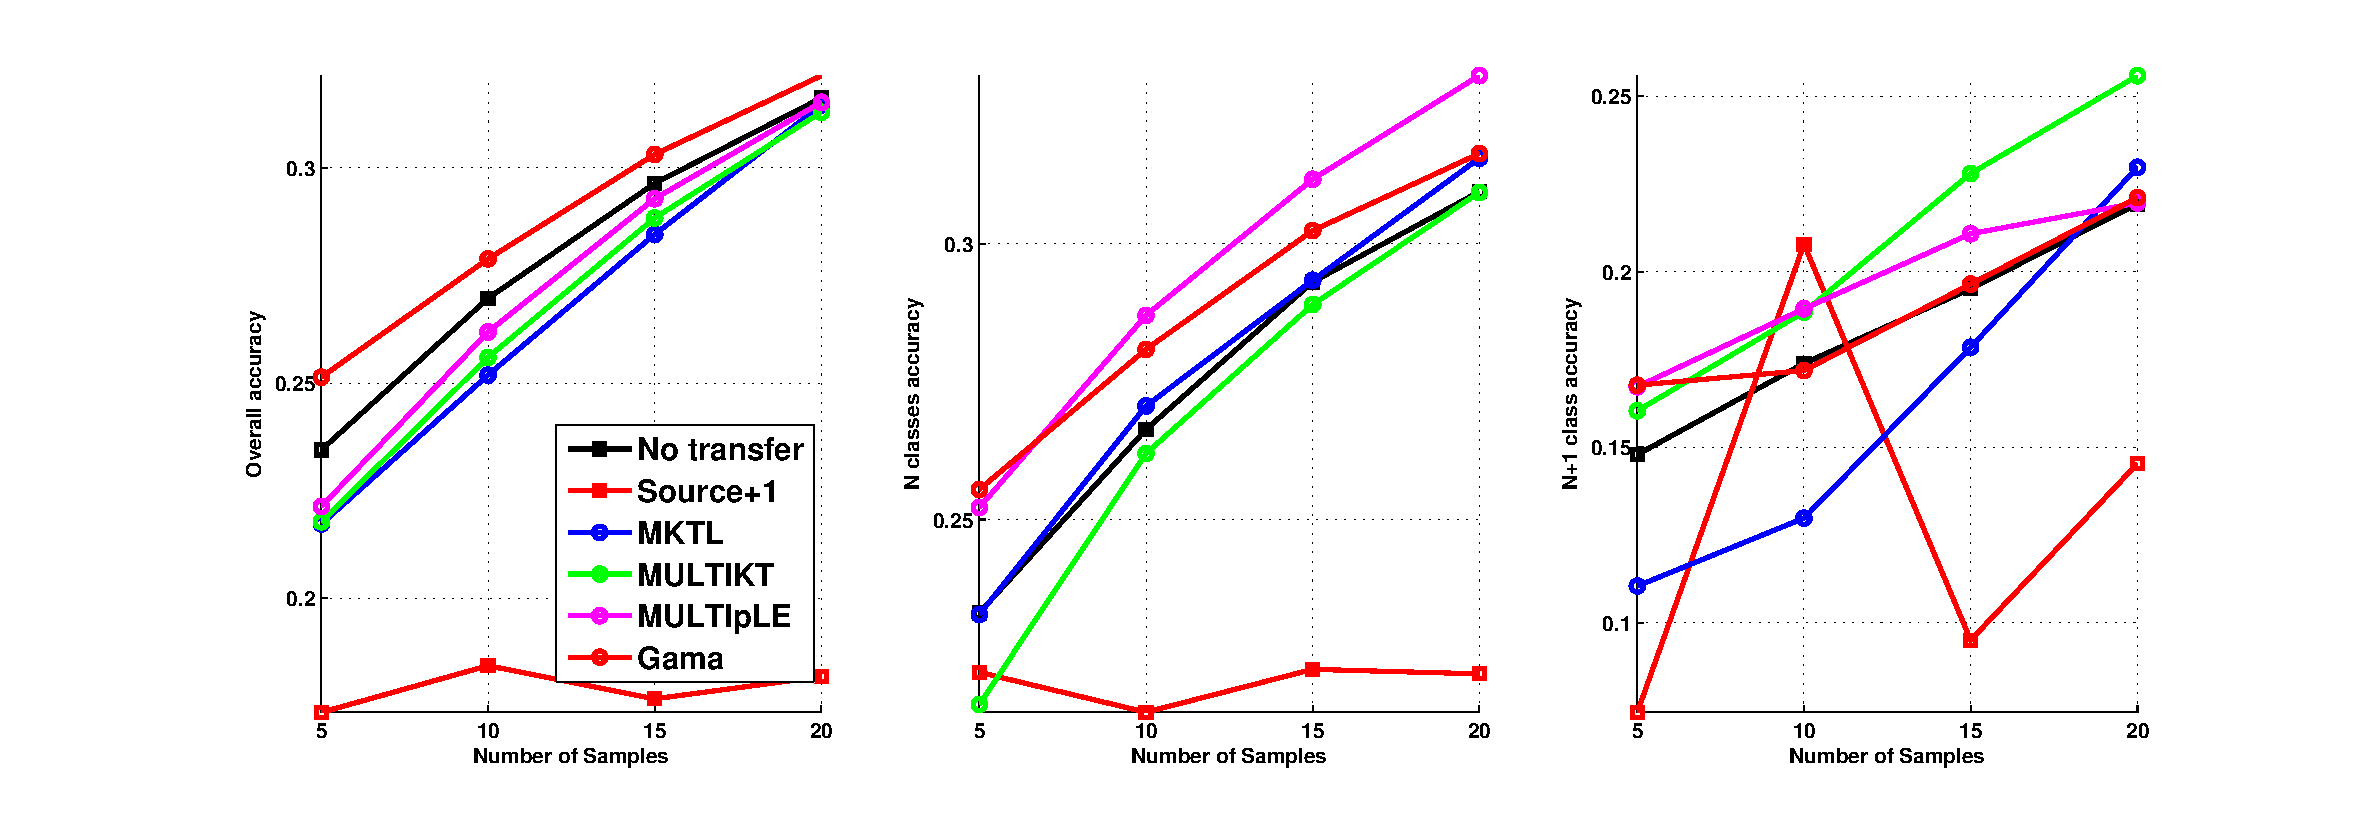
\includegraphics[width=\textwidth,height=5cm]{fig/A2A_MIX_L6_2345.eps}
\caption{Experiment leave class 6 as new category. 2345 as bad class}
\end{figure*}


\section{Conclusion}

% An example of a floating figure using the graphicx package.
% Note that \label must occur AFTER (or within) \caption.
% For figures, \caption should occur after the \includegraphics.
% Note that IEEEtran v1.7 and later has special internal code that
% is designed to preserve the operation of \label within \caption
% even when the captionsoff option is in effect. However, because
% of issues like this, it may be the safest practice to put all your
% \label just after \caption rather than within \caption{}.
%
% Reminder: the "draftcls" or "draftclsnofoot", not "draft", class
% option should be used if it is desired that the figures are to be
% displayed while in draft mode.
%
%\begin{figure}[!t]
%\centering
%\includegraphics[width=2.5in]{myfigure}
% where an .eps filename suffix will be assumed under latex,
% and a .pdf suffix will be assumed for pdflatex; or what has been declared
% via \DeclareGraphicsExtensions.
%\caption{Simulation Results}
%\label{fig_sim}
%\end{figure}

% Note that IEEE typically puts floats only at the top, even when this
% results in a large percentage of a column being occupied by floats.


% An example of a double column floating figure using two subfigures.
% (The subfig.sty package must be loaded for this to work.)
% The subfigure \label commands are set within each subfloat command, the
% \label for the overall figure must come after \caption.
% \hfil must be used as a separator to get equal spacing.
% The subfigure.sty package works much the same way, except \subfigure is
% used instead of \subfloat.
%
%\begin{figure*}[!t]
%\centerline{\subfloat[Case I]\includegraphics[width=2.5in]{subfigcase1}%
%\label{fig_first_case}}
%\hfil
%\subfloat[Case II]{\includegraphics[width=2.5in]{subfigcase2}%
%\label{fig_second_case}}}
%\caption{Simulation results}
%\label{fig_sim}
%\end{figure*}
%
% Note that often IEEE papers with subfigures do not employ subfigure
% captions (using the optional argument to \subfloat), but instead will
% reference/describe all of them (a), (b), etc., within the main caption.


% An example of a floating table. Note that, for IEEE style tables, the
% \caption command should come BEFORE the table. Table text will default to
% \footnotesize as IEEE normally uses this smaller font for tables.
% The \label must come after \caption as always.
%
%\begin{table}[!t]
%% increase table row spacing, adjust to taste
%\renewcommand{\arraystretch}{1.3}
% if using array.sty, it might be a good idea to tweak the value of
% \extrarowheight as needed to properly center the text within the cells
%\caption{An Example of a Table}
%\label{table_example}
%\centering
%% Some packages, such as MDW tools, offer better commands for making tables
%% than the plain LaTeX2e tabular which is used here.
%\begin{tabular}{|c||c|}
%\hline
%One & Two\\
%\hline
%Three & Four\\
%\hline
%\end{tabular}
%\end{table}


% Note that IEEE does not put floats in the very first column - or typically
% anywhere on the first page for that matter. Also, in-text middle ("here")
% positioning is not used. Most IEEE journals/conferences use top floats
% exclusively. Note that, LaTeX2e, unlike IEEE journals/conferences, places
% footnotes above bottom floats. This can be corrected via the \fnbelowfloat
% command of the stfloats package.








% conference papers do not normally have an appendix


% use section* for acknowledgement
\section*{Acknowledgment}

%\appendices
%\input{appendix.tex}







% trigger a \newpage just before the given reference
% number - used to balance the columns on the last page
% adjust value as needed - may need to be readjusted if
% the document is modified later
%\IEEEtriggeratref{8}
% The "triggered" command can be changed if desired:
%\IEEEtriggercmd{\enlargethispage{-5in}}

% references section

% can use a bibliography generated by BibTeX as a .bbl file
% BibTeX documentation can be easily obtained at:
% http://www.ctan.org/tex-archive/biblio/bibtex/contrib/doc/
% The IEEEtran BibTeX style support page is at:
% http://www.michaelshell.org/tex/ieeetran/bibtex/
%\bibliographystyle{IEEEtran}
% argument is your BibTeX string definitions and bibliography database(s)
%\bibliography{IEEEabrv,../bib/paper}
%
% <OR> manually copy in the resultant .bbl file
% set second argument of \begin to the number of references
% (used to reserve space for the reference number labels box)
\bibliographystyle{IEEEtran}
\bibliography{research}




% that's all folks
\end{document}


